\begin{figure*}[t]
  \centering
  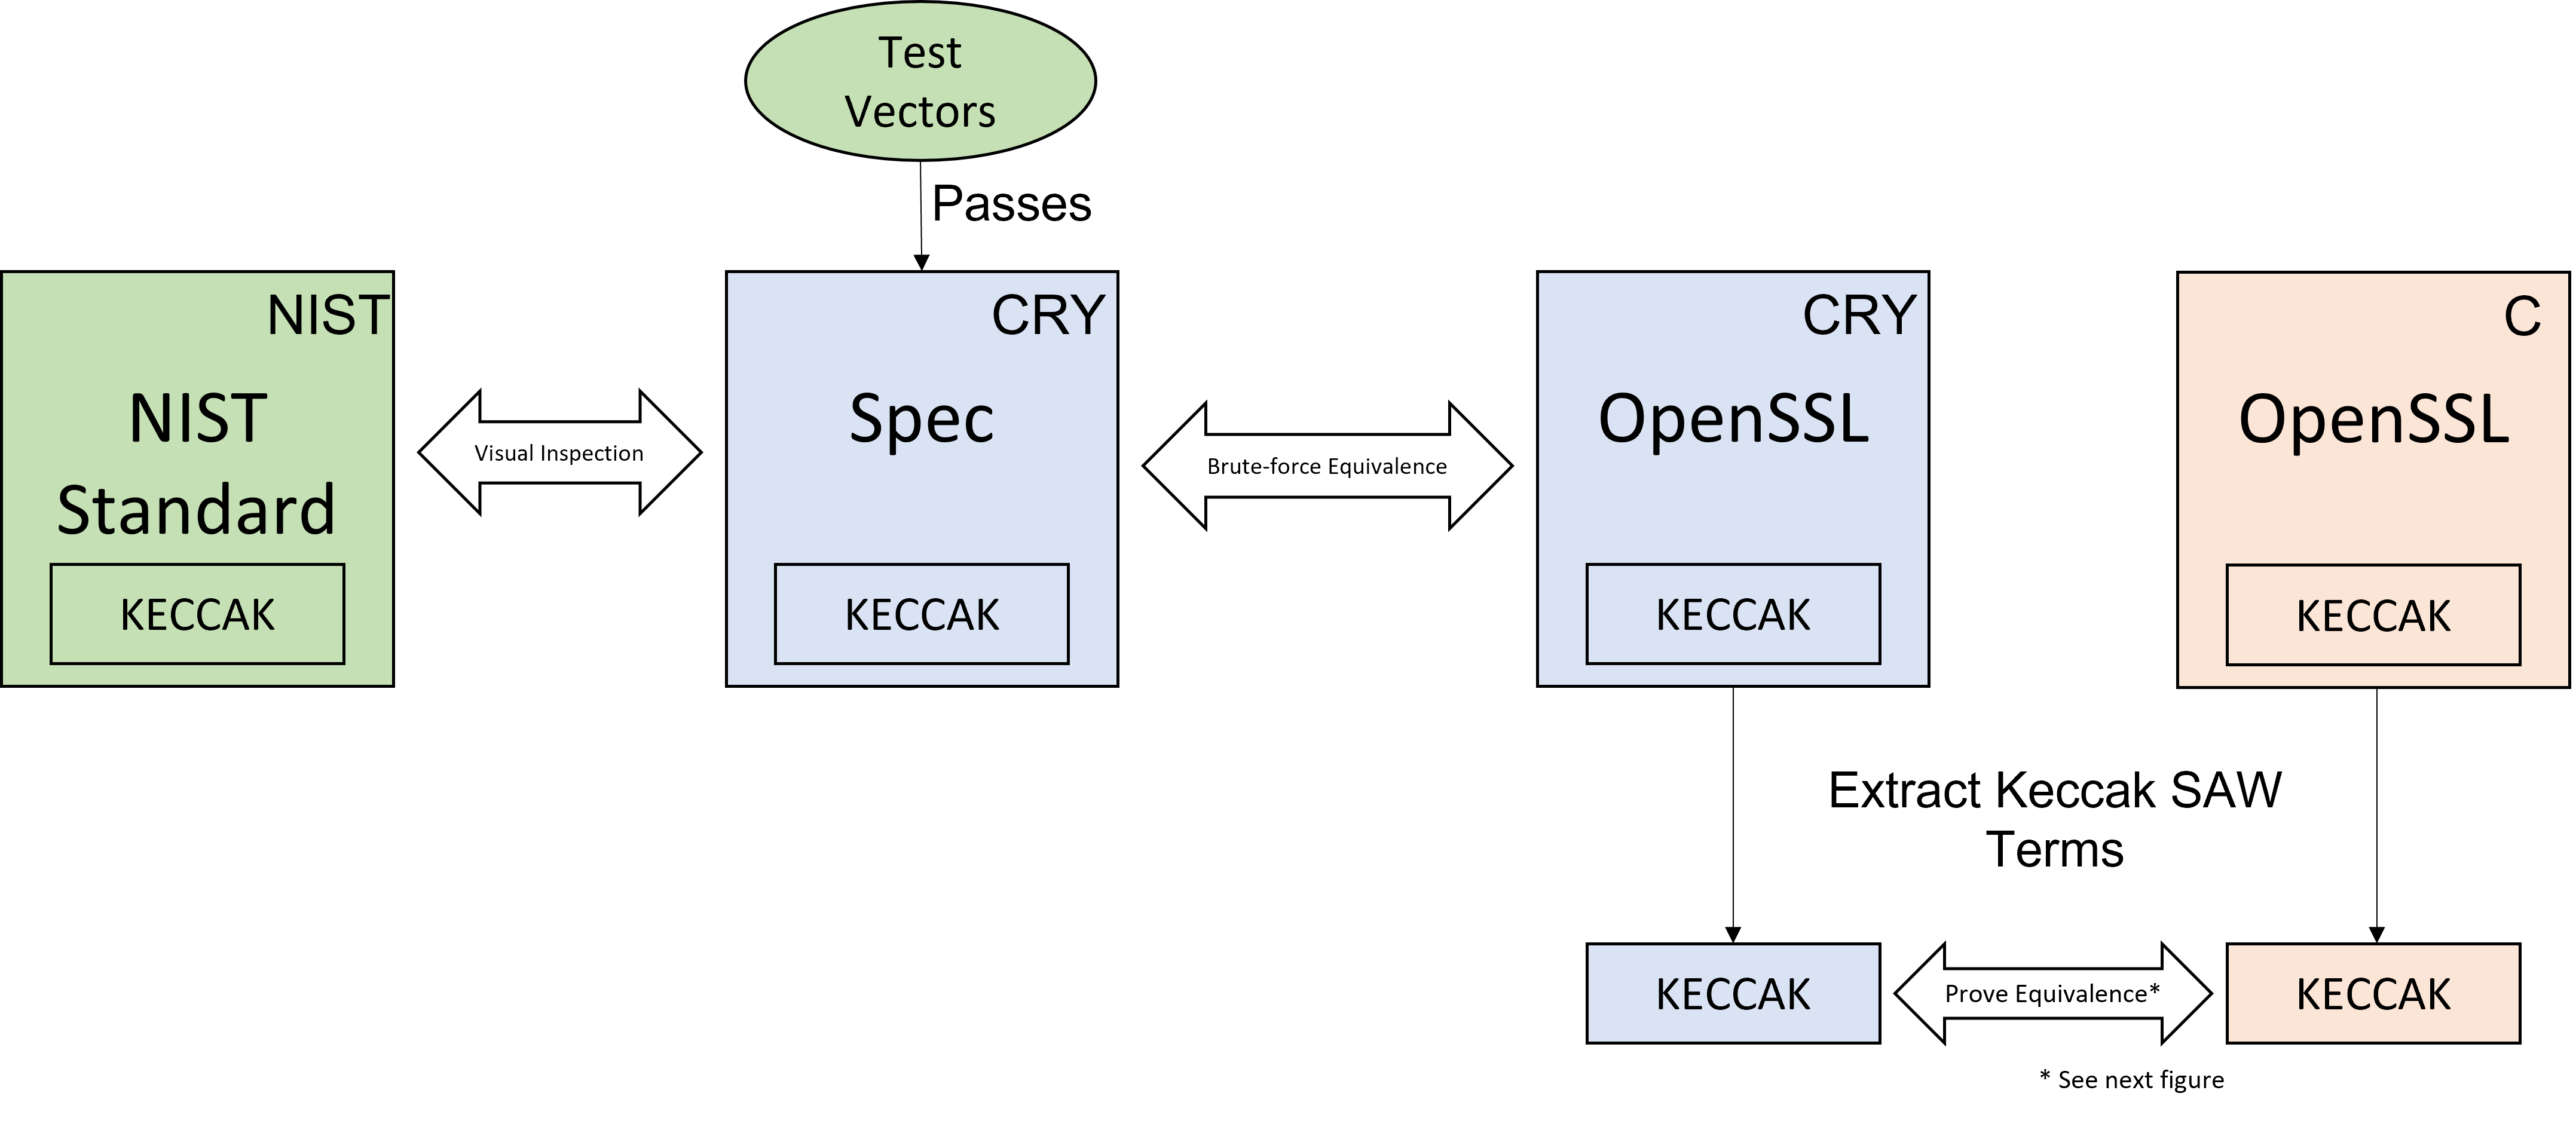
\includegraphics[width=\linewidth]{figs/proof.png}
  
  \caption{Equivalence proof for the \shaThree\ standard and the \openssl\ C implementation.}
  \label{fig:proofStructure}
  
\end{figure*}

The goal of the work presented in this paper is to prove the \openssl\ implementation of \shaThree\ matches the \fips\ publication by \nist.
\figref{fig:proofStructure} illustrates the proof strategy.
The proof begins on the left of the figure with the box labeled \emph{NIST Standard}. 
This box represents the \fips\ standard that defines the \shaThree\ algorithm with english prose and math.
The standard also provides several test inputs with the correspondingly  expected digests.
The first step of the proof reproduces the \fips\ \shaThree\ description in \cryptol.
That is the box to the right of the \emph{NIST Standard} box labeled \emph{Spec}.

The equivalence between the \fips\ standard and the \cryptol\ specification is argued by visual inspection along with tests over the published test vectors with their expected digests.
\shaThree\ is described algorithmically in the standard making use of universal quantifiers and other looping structures in the definition.
\cryptol\ is functional in that it uses list comprehensions for iteration, and it does not have quantifiers.
Visually certifying a specification of \shaThree\ that uses list comprehensions directly for quantification and looping is difficult at best---the list comprehensions are too complex to read, and they obscure the algorithmic, and mathematic, structure in the published standard.

The syntactic disconnect between the quantification and looping in the published standard and the list comprehensions in the \cryptol\ specification is bridged with a library that hides the list comprehensions with appropriately named functions.
The final specification with the function hiding the list comprehensions has a one-to-one correspondence to the published standard that is easy to visually certify.
The specification is further validated by tests in \cryptol\ over the published test vectors.
The digests computed from the \cryptol\ specification exactly match those published in the standard on each given input.
The equivalence arrow between the \emph{NIST Standard} box and the \emph{Spec} box represents the visual certification and test vector results.
\secref{sec:fips} details the specification and library.

The extracted core term from the \openssl\ C implementation of \shaThree\ is too big and complex for \saw\ to reason about directly.
Adding to the complexity of the equivalence proof is that the \openssl\ implementation changes the meaning of the state $S$ in the algorithm so that it no longer directly matches the meaning defined in the published standard.
The change effectively reorders the matrix definition of the state to be more amenable to memory and aspects of the \keccak\ implementation in C.
The change is significant enough to make it extremely difficult to argue manually that the computation implemented in \openssl\ matches that defined in the standard.

The next step of the equivalence proof creates a \cryptol\ specification that matches the state reordering in the \openssl\ implementation in an effort to show an equivalence between it and the \cryptol\ specification for the standard.
This new specification is the box in the right middle of \figref{fig:proofStructure} labeled \emph{OpenSSL} with the \emph{CRY} annotation in the upper right corner.
\saw\ is not able to reason symbolically about input and digest sizes to construct a general proof of equivalence between the published standard and the \openssl\ \cryptol specifications, but it is able to prove equivalence between the two specifications given specific sizes for the input and digest.

A series of \saw\ proofs over a range of input sizes with a digest size fixed at $256$-bits is used to prove the equivalence between the published standard and the \openssl\ \cryptol specifications.
The series of proofs varies the input size from zero bits to $1,087$ bits to reflect the rate $1,088$ bit rate required for a 256-bit digest.
The proofs establish the correctness of the input padding and covers the situation where the padding adds an additional $1,088$-bit block to the input 
As such, the meaning of the equivalence arrow between the \emph{Spec} box and the \emph{OpenSSL} box in the middle of the figure is that the two specifications have equivalent computation for a $256$-bit digest for message sizes from $0$ bits to $1,087$ bits.

\begin{figure*}[t]
  \centering
  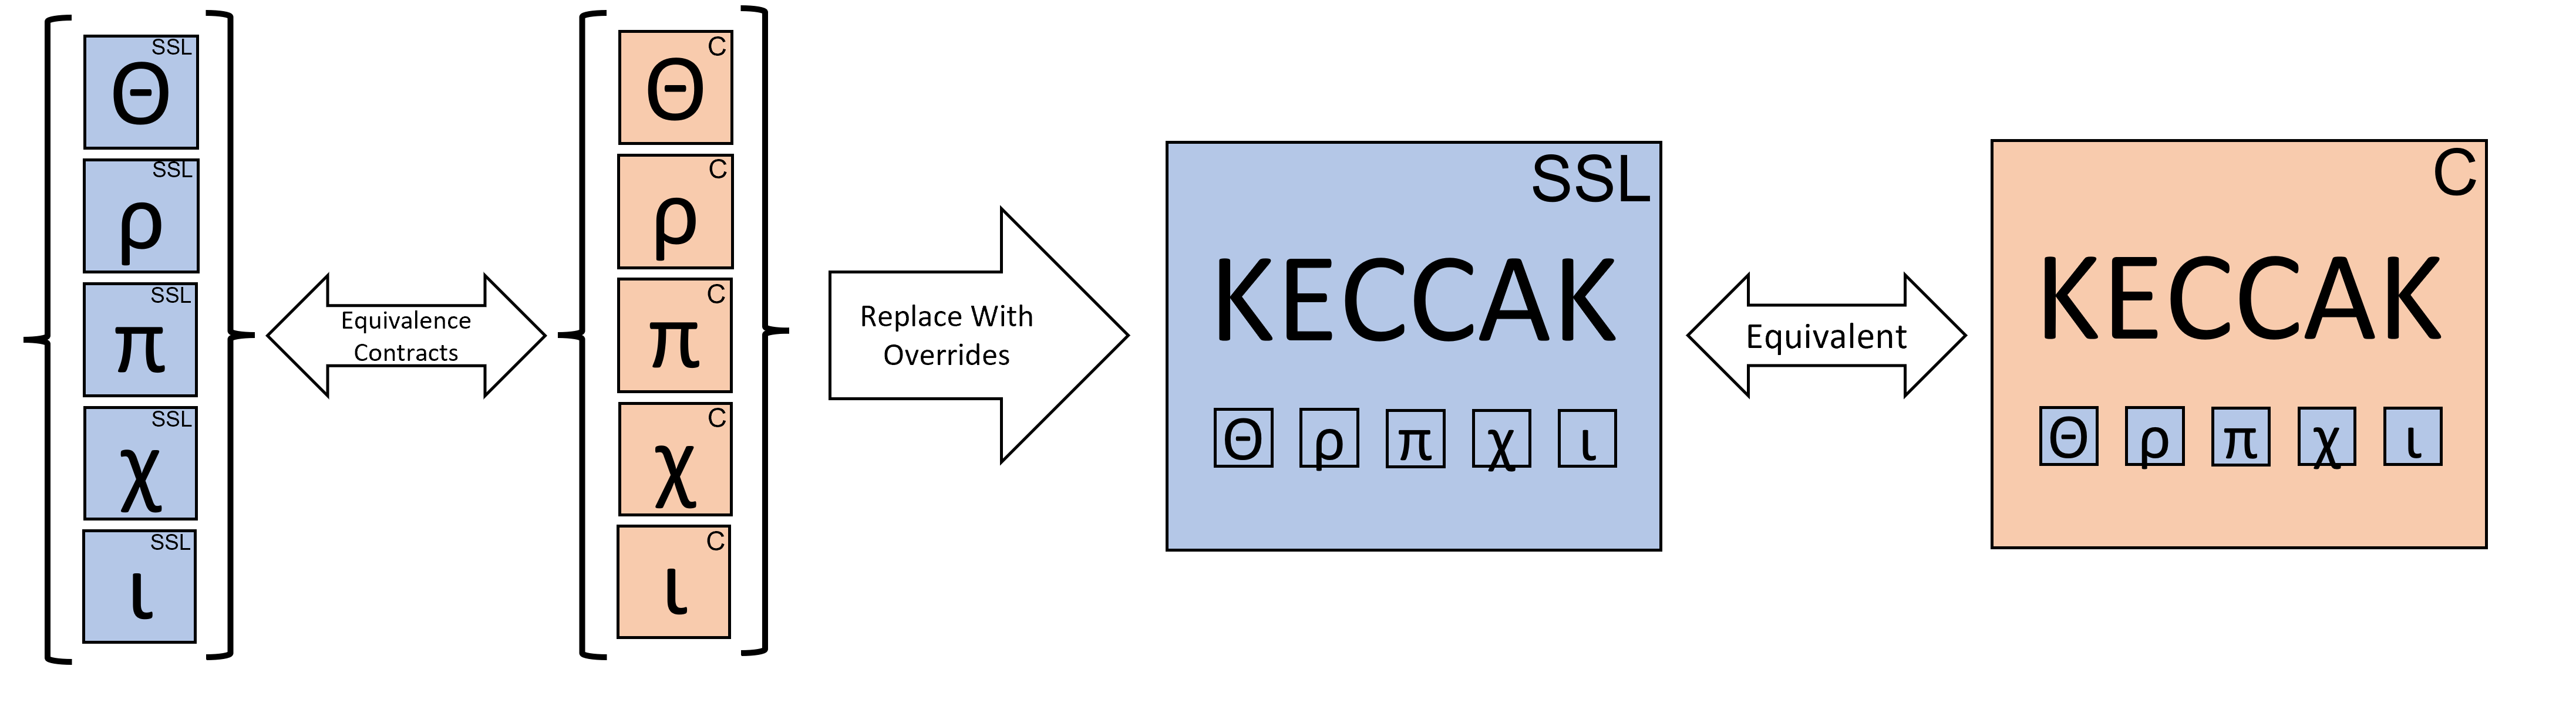
\includegraphics[width=\linewidth]{figs/proof2.png}
  
  \caption{Inner Function Contracts}
  \label{fig:proofStructure2}
  
\end{figure*}

The rest of the equivalence proof between the standard and the \openssl\ implementation centers on the \keccak\ algorithm as shown in the bottom right of \figref{fig:proofStructure}.
The meaning of the equivalence arrow between the \keccak\ definition in the \cryptol\ specification based on the \openssl\ implementation and the actual implemented \keccak\ algorithm in the \openssl\ C implementation is that their computation exactly matches for any input state.
That proof cannot be constructed directly by \saw\ since the extracted core term from the C implementation is too big for symbolic execution when considering all twenty-four rounds required by \keccak.
The full proof requires overrides.

The proof of equivalence between the specification of \keccak\ and the C implementation of \keccak\ in \openssl\ relies on overrides in \saw as shown in \figref{fig:proofStructure2}.
Here, \saw\ proves equivalence between the \cryptol\ specification and the C implementation for each of the five functions that comprise one round of \keccak\ given some arbitrary input state.
That is the meaning of the right hand side of \figref{fig:proofStructure2}.
These are equivalent on any input.

The implementations for each of the five \keccak\ functions in the C implementation are replaced by the corresponding equivalent \cryptol\ specifications in the extracted model from C.
\saw\ is then able to prove the C implementation of \keccak equivalent to the \cryptol\ specification of the \openssl\ implementation of \keccak\ over all twenty-four rounds for any arbitrary input state.
The equivalence is independent of the digest size, message size, or state.

%% TODO: update the figure and text with results from the proof of the padding and the squeeze functions.

In summary, the \cryptol\ specification of the \fips\ standard relies on visual inspection and test vectors for equivalence.
The equivalence between the \cryptol\ specification of the standard and the \cryptol\ specification of \openssl's implementation is limited to the 256-bit digest on input sizes from $0$ bits to $1,087$ bits.
That is a proof that considers all of \algoref{alg:sha3}.
The equivalence between \openssl\ \cryptol\ specification and the actual C implementation is limited to the \keccak algorithm only.
That is a proof that only considers \lineref{line:keccak} in \algoref{alg:sha3} but holds for any state and is independent of the digest size and rate.

%% TODO: summarize the cost of the total proof in terms of time and identify the machine used for the proof.
